\documentclass[a4paper,11pt]{article}

\usepackage[a4paper,margin=1.9cm]{geometry}
\usepackage[T1]{fontenc}
\usepackage{hyperref}
\usepackage[table]{xcolor}
\usepackage{booktabs}
\usepackage{tabularx}
\usepackage{array}
\usepackage{fancyhdr}
\usepackage{listings}
\usepackage{graphicx}
\usepackage{tikz}
\usepackage{microtype}

\usetikzlibrary{arrows.meta,positioning,shapes.geometric}

\hypersetup{
  colorlinks=true,
  linkcolor=blue!60!black,
  urlcolor=blue!60!black,
  pdftitle={Kubernetes Minikube Guide},
  pdfauthor={OpenAI Codex}
}

\definecolor{panel}{HTML}{F7F4EC}
\definecolor{skywash}{HTML}{EAF4FF}
\definecolor{mintwash}{HTML}{EAF9F1}
\definecolor{sunwash}{HTML}{FFF5D6}
\definecolor{rosewash}{HTML}{FCECEF}
\definecolor{ink}{HTML}{22303C}
\definecolor{warm}{HTML}{A55C36}
\definecolor{codebg}{HTML}{FBFBFB}
\definecolor{coderule}{HTML}{D8D8D8}
\definecolor{softblue}{HTML}{3B6EA5}
\definecolor{softgreen}{HTML}{2C8C61}
\definecolor{softorange}{HTML}{C97924}

\pagestyle{fancy}
\fancyhf{}
\lhead{Kubernetes Minikube Guide}
\rhead{\thepage}
\setlength{\headheight}{14pt}

\newcolumntype{Y}{>{\raggedright\arraybackslash}X}

\lstdefinestyle{code}{
  backgroundcolor=\color{codebg},
  frame=single,
  rulecolor=\color{coderule},
  basicstyle=\ttfamily\small,
  keywordstyle=\color{softblue}\bfseries,
  commentstyle=\color{softgreen},
  stringstyle=\color{softorange},
  showstringspaces=false,
  breaklines=true,
  columns=fullflexible
}

\lstdefinestyle{terminal}{
  backgroundcolor=\color{black!3},
  frame=single,
  rulecolor=\color{black!20},
  basicstyle=\ttfamily\small,
  showstringspaces=false,
  breaklines=true,
  columns=fullflexible
}

\newcommand{\PanelBox}[1]{%
  \begin{center}
  \fcolorbox{black!35}{panel}{\parbox{0.95\linewidth}{#1}}
  \end{center}
}

\newcommand{\LearningCallout}[2]{%
  \begin{center}
  \fcolorbox{black!35}{#1}{\parbox{0.95\linewidth}{#2}}
  \end{center}
}

\newcommand{\MemoryBox}[1]{%
  \LearningCallout{skywash}{\textbf{Memory hook.} #1}
}

\newcommand{\ExerciseBox}[1]{%
  \LearningCallout{mintwash}{\textbf{Active learning.} #1}
}

\newcommand{\PitfallBox}[1]{%
  \LearningCallout{rosewash}{\textbf{Common mistake.} #1}
}

\newcommand{\BigPictureFigure}{%
\begin{center}
\resizebox{0.96\linewidth}{!}{%
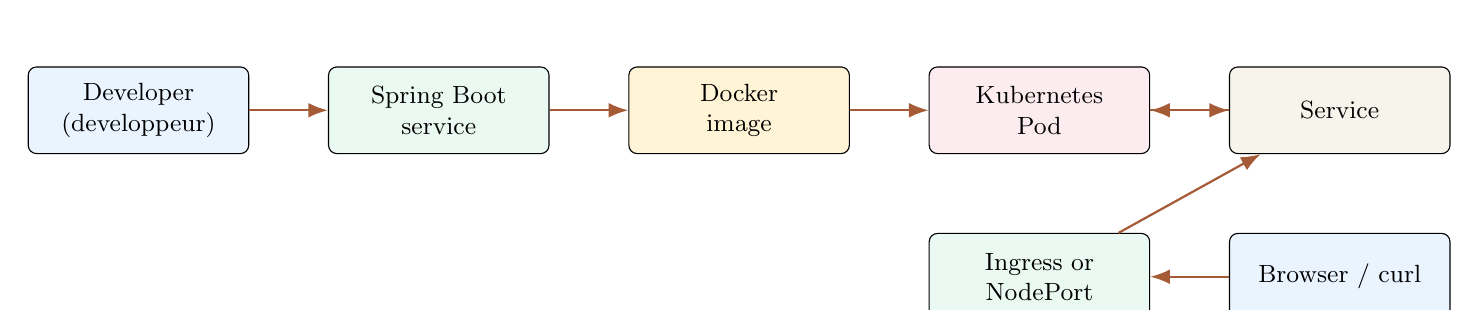
\begin{tikzpicture}[
  node distance=10mm and 10mm,
  every node/.style={font=\small, align=center},
  box/.style={draw=black, rounded corners=3pt, minimum height=11mm, minimum width=28mm},
  arr/.style={-{Latex[length=2.5mm]}, thick, draw=warm}
]
\node[box, fill=skywash] (dev) {Developer\\(developpeur)};
\node[box, fill=mintwash, right=of dev] (code) {Spring Boot\\service};
\node[box, fill=sunwash, right=of code] (docker) {Docker\\image};
\node[box, fill=rosewash, right=of docker] (pod) {Kubernetes\\Pod};
\node[box, fill=panel, right=of pod] (svc) {Service};
\node[box, fill=skywash, below=of svc] (browser) {Browser / curl};
\node[box, fill=mintwash, left=of browser] (ing) {Ingress or\\NodePort};
\draw[arr] (dev) -- (code);
\draw[arr] (code) -- (docker);
\draw[arr] (docker) -- (pod);
\draw[arr] (pod) -- (svc);
\draw[arr] (browser) -- (ing);
\draw[arr] (ing) -- (svc);
\draw[arr] (svc) -- (pod);
\end{tikzpicture}
}
\end{center}
}

\newcommand{\KubernetesObjectsFigure}{%
\begin{center}
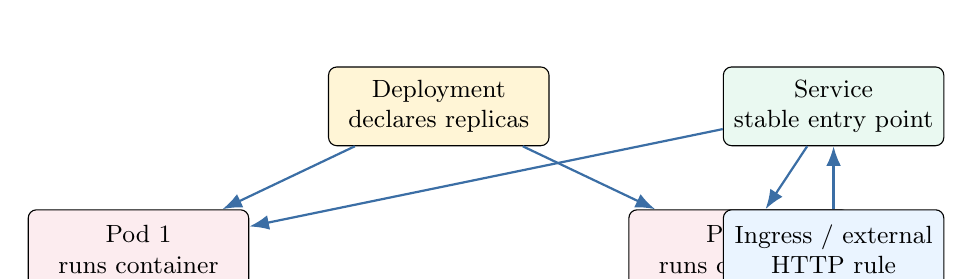
\begin{tikzpicture}[
  node distance=8mm and 10mm,
  every node/.style={font=\small, align=center},
  box/.style={draw=black, rounded corners=3pt, minimum height=10mm, minimum width=28mm},
  arr/.style={-{Latex[length=2.5mm]}, thick, draw=softblue}
]
\node[box, fill=sunwash] (deployment) {Deployment\\declares replicas};
\node[box, fill=rosewash, below left=of deployment] (pod1) {Pod 1\\runs container};
\node[box, fill=rosewash, below right=of deployment] (pod2) {Pod 2\\runs container};
\node[box, fill=mintwash, right=22mm of deployment] (service) {Service\\stable entry point};
\node[box, fill=skywash, below=of service] (ingress) {Ingress / external\\HTTP rule};
\draw[arr] (deployment) -- (pod1);
\draw[arr] (deployment) -- (pod2);
\draw[arr] (service) -- (pod1);
\draw[arr] (service) -- (pod2);
\draw[arr] (ingress) -- (service);
\end{tikzpicture}
\end{center}
}

\newcommand{\RequestFlowFigure}{%
\begin{center}
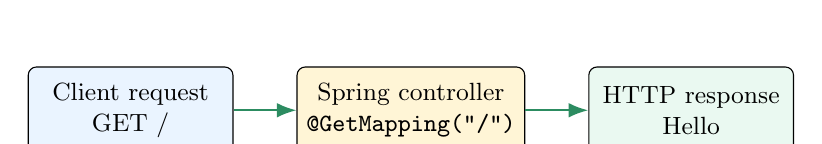
\begin{tikzpicture}[
  node distance=9mm and 8mm,
  every node/.style={font=\small, align=center},
  box/.style={draw=black, rounded corners=3pt, minimum height=11mm, minimum width=26mm},
  arr/.style={-{Latex[length=2.5mm]}, thick, draw=softgreen}
]
\node[box, fill=skywash] (client) {Client request\\GET /};
\node[box, fill=sunwash, right=of client] (controller) {Spring controller\\\texttt{@GetMapping("/")} };
\node[box, fill=mintwash, right=of controller] (response) {HTTP response\\Hello};
\draw[arr] (client) -- (controller);
\draw[arr] (controller) -- (response);
\end{tikzpicture}
\end{center}
}

\title{\textbf{Kubernetes Minikube Project Guide}\\[0.5em]
\large A complete A4 learning document for the repository\\
\texttt{kubernetes-minikube}}
\author{Prepared from the project files for self-study}
\date{\today}

\begin{document}
\maketitle
\tableofcontents
\newpage

\section{Introduction}

This document explains the repository \texttt{kubernetes-minikube} as a complete learning object. The goal is not only to say what the commands do, but to explain why the project matters in distributed programming (\emph{programmation distribuee}), what each source file contributes, how requests move through the system, and how to reason about Docker, Kubernetes, services, ingress, and scaling.

\PanelBox{
\textbf{Short answer: what is this project?}\\
It is a minimal Spring Boot web service packaged into a Docker image and deployed into a local Kubernetes cluster provided by Minikube. The service itself is simple and returns \texttt{Hello}, but the infrastructure around it teaches real distributed-systems ideas: packaging, scheduling, replication, service abstraction, and external exposure.
}

\subsection{Why this belongs to distributed programming}

At first glance, the application code is tiny. That can make the project look too simple. In reality, the educational value is in the deployment model:

\begin{itemize}
  \item the service runs in a container instead of directly on your host machine,
  \item Kubernetes decides where the container runs and how many copies should exist,
  \item a Service offers a stable network identity even when Pods are replaced,
  \item an Ingress or NodePort exposes the application to the outside world,
  \item scaling creates multiple instances of the same service, which is a core distributed-systems concern.
\end{itemize}

\MemoryBox{A distributed program is not only about writing multiple classes. It is about computation spread across network boundaries, runtime boundaries, and independently managed execution units.}

\subsection{The main learning promise of this repository}

If you understand this repository deeply, you understand the first complete local path from code to distributed deployment:

\begin{enumerate}
  \item write a service,
  \item package it,
  \item containerize it,
  \item deploy it,
  \item expose it,
  \item scale it,
  \item reason about traffic and availability.
\end{enumerate}

\BigPictureFigure

\section{Repository Map}

\begin{center}
\begin{tabularx}{\textwidth}{@{}lY@{}}
\toprule
\textbf{File} & \textbf{Role in the project} \\
\midrule
\texttt{README.md} & installation, Docker, Minikube, deployment, exposure, and scaling workflow \\
\texttt{MyService/build.gradle} & Java and Spring Boot build configuration \\
\texttt{MyService/src/main/java/.../MyServiceApplication.java} & Spring Boot entry point \\
\texttt{MyService/src/main/java/.../MyServiceRest.java} & REST controller that returns \texttt{Hello} \\
\texttt{MyService/src/test/java/.../MyserviceApplicationTests.java} & minimal Spring Boot context test \\
\texttt{MyService/Dockerfile} & multi-stage container build and runtime image \\
\texttt{myservice-deployment.yml} & Kubernetes Deployment definition \\
\texttt{myservice-service.yml} & Kubernetes NodePort Service definition \\
\texttt{myservice-loadbalancing-service.yml} & Kubernetes LoadBalancer Service definition \\
\texttt{ingress.yml} & Kubernetes Ingress definition \\
\bottomrule
\end{tabularx}
\end{center}

\section{The Architecture of the Project}

\KubernetesObjectsFigure

\subsection{The runtime story}

The runtime chain is:

\begin{enumerate}
  \item Java code starts a Spring Boot HTTP server.
  \item Docker packages that server with a Java runtime.
  \item Kubernetes creates a Pod containing the container.
  \item A Service gives that Pod set a stable address.
  \item An Ingress or NodePort lets external traffic reach the Service.
\end{enumerate}

\subsection{Why each layer exists}

\begin{center}
\begin{tabularx}{\textwidth}{@{}lY@{}}
\toprule
\textbf{Layer} & \textbf{Reason} \\
\midrule
Application & defines the business behavior, here a simple HTTP response \\
Container & makes the runtime reproducible across machines \\
Deployment & declares the desired number of running instances \\
Service & hides Pod ephemerality behind a stable access point \\
Ingress & routes external HTTP traffic by host and path \\
\bottomrule
\end{tabularx}
\end{center}

\section{Code Walkthrough: Application Layer}

\subsection{The build file: \texttt{build.gradle}}

\begin{lstlisting}[style=code, language=Java, caption={build.gradle}]
plugins {
    id 'java'
    id 'org.springframework.boot' version '3.2.0'
    id 'io.spring.dependency-management' version '1.1.4'
}

group = 'com.example'
version = '0.0.1-SNAPSHOT'
sourceCompatibility = '21'

java {
    toolchain {
        languageVersion = JavaLanguageVersion.of(21)
    }
}

repositories {
    mavenCentral()
}

dependencies {
    implementation 'org.springframework.boot:spring-boot-starter-web'
    testImplementation 'org.springframework.boot:spring-boot-starter-test'
}

tasks.named('test') {
    useJUnitPlatform()
}
\end{lstlisting}

\textbf{What this file does.}

\begin{itemize}
  \item The \texttt{plugins} block activates Java support and Spring Boot support.
  \item \texttt{sourceCompatibility = '21'} means the code targets Java 21.
  \item The \texttt{toolchain} section asks Gradle for Java 21 even if the local default JDK differs.
  \item \texttt{mavenCentral()} is the remote package repository.
  \item \texttt{spring-boot-starter-web} adds Spring MVC, embedded Tomcat, and HTTP features.
  \item \texttt{spring-boot-starter-test} adds testing tools for Spring and JUnit.
  \item \texttt{useJUnitPlatform()} tells Gradle to run tests with JUnit 5.
\end{itemize}

\MemoryBox{The build file is the contract between your source code and the toolchain. Without it, the project does not know which libraries to download or how to assemble the application.}

\subsection{The application entry point}

\begin{lstlisting}[style=code, language=Java, caption={MyServiceApplication.java}]
package com.example.myservice;

import org.springframework.boot.SpringApplication;
import org.springframework.boot.autoconfigure.SpringBootApplication;

@SpringBootApplication
public class MyServiceApplication {

    public static void main(String[] args) {
        SpringApplication.run(MyServiceApplication.class, args);
    }

}
\end{lstlisting}

\textbf{Line-by-line explanation.}

\begin{itemize}
  \item \texttt{package com.example.myservice;} organizes the class inside a Java namespace.
  \item \texttt{@SpringBootApplication}\\
  is a meta-annotation that enables component scanning, auto-configuration, and Spring Boot startup behavior.
  \item \texttt{main(...)} is the standard Java entry method.
  \item \texttt{SpringApplication.run(...)} boots the Spring container and starts the embedded web server.
\end{itemize}

\ExerciseBox{
\textbf{Question.} Why do we need a framework bootstrap class instead of writing only the controller?\\
\textbf{Reasoned answer.} The controller defines request behavior, but something still has to start the application context, build the HTTP server, scan components, and wire the dependencies. The bootstrap class performs that system-level startup role.
}

\subsection{The REST controller}

\RequestFlowFigure

\begin{lstlisting}[style=code, language=Java, caption={MyServiceRest.java}]
package com.example.myservice;

import org.springframework.web.bind.annotation.GetMapping;
import org.springframework.web.bind.annotation.RestController;

@RestController
public class MyServiceRest {

    @GetMapping("/")
    public String sayHello(){
        return "Hello";
    }

}
\end{lstlisting}

\textbf{Detailed explanation.}

\begin{itemize}
  \item \texttt{@RestController} means this class handles HTTP requests and returns response bodies directly.
  \item \texttt{@GetMapping("/")} binds the method to HTTP \texttt{GET} requests on the root path.
  \item \texttt{public String sayHello()} is the method called when the route matches.
  \item \texttt{return "Hello";} becomes the HTTP response body.
\end{itemize}

\begin{lstlisting}[style=terminal, caption={Visible result in a browser or with curl}]
$ curl http://localhost:8080/
Hello
\end{lstlisting}

\MemoryBox{This controller is simple on purpose. The course idea is: keep the business logic small so you can focus on the distributed infrastructure around it.}

\subsection{The test class}

\begin{lstlisting}[style=code, language=Java, caption={MyserviceApplicationTests.java}]
package com.example.myservice;

import org.junit.jupiter.api.Test;
import org.springframework.boot.test.context.SpringBootTest;

@SpringBootTest
class MyserviceApplicationTests {

    @Test
    void contextLoads() {
    }

}
\end{lstlisting}

\textbf{What this test means.}

This test does not verify endpoint output. It verifies something more basic: can the Spring application context start correctly? If this test fails, the application wiring is broken.

\PitfallBox{Students often think an empty test is useless. Here the emptiness is intentional: the test passes only if Spring can construct the application context without configuration errors.}

\section{Code Walkthrough: Container Layer}

\subsection{The Dockerfile}

\begin{lstlisting}[style=code, caption={MyService/Dockerfile}]
# Stage 1: Build
FROM gradle:8.5-jdk21 AS build
WORKDIR /app
COPY build.gradle settings.gradle ./
COPY src ./src
RUN gradle build --no-daemon -x test

# Stage 2: Run
FROM eclipse-temurin:21-jre
WORKDIR /app
COPY --from=build /app/build/libs/*.jar app.jar
EXPOSE 8080
ENTRYPOINT ["java", "-jar", "app.jar"]
\end{lstlisting}

\textbf{Why this is a multi-stage build.}

\begin{itemize}
  \item Stage 1 uses a heavier image with Gradle and a full JDK to compile the application.
  \item Stage 2 uses a lighter JRE-only image to run the built jar.
  \item This reduces the final image size and removes unnecessary build tools from production.
\end{itemize}

\textbf{Line-by-line explanation.}

\begin{itemize}
  \item \texttt{FROM gradle:8.5-jdk21 AS build}: create a build stage named \texttt{build}.
  \item \texttt{WORKDIR /app}: all following commands run relative to \texttt{/app}.
  \item \texttt{COPY build.gradle settings.gradle ./}: copy build metadata first.
  \item \texttt{COPY src ./src}: copy source files.
  \item \texttt{RUN gradle build --no-daemon -x test}: build the jar, skip tests.
  \item \texttt{FROM eclipse-temurin:21-jre}: switch to a runtime-only base image.
  \item \texttt{COPY --from=build ...}: copy the built jar from the first stage.
  \item \texttt{EXPOSE 8080}: document the container port.
  \item \texttt{ENTRYPOINT [...]}: define the command that runs when the container starts.
\end{itemize}

\begin{lstlisting}[style=terminal, caption={Build and run flow}]
$ docker build -t myservice .
$ docker run -p 4000:8080 myservice
\end{lstlisting}

\begin{lstlisting}[style=terminal, caption={Visible result}]
$ curl http://localhost:4000/
Hello
\end{lstlisting}

\section{Code Walkthrough: Kubernetes Layer}

\subsection{Deployment manifest}

\begin{lstlisting}[style=code, caption={myservice-deployment.yml}]
apiVersion: apps/v1
kind: Deployment
metadata:
  name: myservice
spec:
  replicas: 1
  selector:
    matchLabels:
      app: myservice
  template:
    metadata:
      labels:
        app: myservice
    spec:
      containers:
        - image: efrei/myservice:1
          imagePullPolicy: IfNotPresent
          name: myservice
      restartPolicy: Always
\end{lstlisting}

\textbf{What a Deployment does.}

A Deployment declares the desired state (\emph{etat desire}) of the application: how many replicas should exist, which container image should run, and which labels identify the Pods.

\textbf{Important fields.}

\begin{itemize}
  \item \texttt{apiVersion: apps/v1}: use the Kubernetes Deployment API.
  \item \texttt{kind: Deployment}: this object manages replica lifecycle.
  \item \texttt{metadata.name}: human-readable cluster name.
  \item \texttt{replicas: 1}: exactly one Pod should exist.
  \item \texttt{selector.matchLabels}: tells the Deployment which Pods belong to it.
  \item \texttt{template.metadata.labels}: labels applied to created Pods.
  \item \texttt{containers}: actual runtime container spec.
  \item \texttt{imagePullPolicy: IfNotPresent}: reuse a cached image when available.
\end{itemize}

\MemoryBox{The Pod IP can change. The Deployment name and labels are stable configuration. This is one reason Kubernetes needs labels and Services.}

\subsection{NodePort service}

\begin{lstlisting}[style=code, caption={myservice-service.yml}]
apiVersion: v1
kind: Service
metadata:
  name: myservice
spec:
  ports:
    - nodePort: 31280
      port: 8080
      protocol: TCP
      targetPort: 8080
  selector:
    app: myservice
  type: NodePort
\end{lstlisting}

\textbf{How to read this file.}

\begin{itemize}
  \item \texttt{kind: Service} creates a stable network endpoint.
  \item \texttt{selector.app: myservice} means ``send traffic to Pods labeled \texttt{app=myservice}''.
  \item \texttt{targetPort: 8080} is the port inside the Pod container.
  \item \texttt{port: 8080} is the Service port inside the cluster.
  \item \texttt{nodePort: 31280} opens a fixed port on the node itself.
  \item \texttt{type: NodePort} chooses this exposure model.
\end{itemize}

\begin{lstlisting}[style=terminal, caption={Expected access pattern}]
Browser -> Minikube node IP:31280 -> Service -> Pod -> Spring controller
\end{lstlisting}

\subsection{LoadBalancer service}

\begin{lstlisting}[style=code, caption={myservice-loadbalancing-service.yml}]
apiVersion: v1
kind: Service
metadata:
  labels:
    app: myservice
  name: myservice
spec:
  ports:
    - nodePort: 30945
      port: 8080
      protocol: TCP
      targetPort: 8080
  selector:
    app: myservice
  type: LoadBalancer
\end{lstlisting}

\textbf{What changes compared with NodePort?}

The selector logic is the same, but the exposure intent changes. A \texttt{LoadBalancer} Service asks the platform to provision an external load balancer. In a real cloud environment this often creates a cloud load balancer resource. In Minikube, this behavior is simulated or adapted depending on addons and tooling.

\subsection{Ingress}

\begin{lstlisting}[style=code, caption={ingress.yml}]
apiVersion: networking.k8s.io/v1
kind: Ingress
metadata:
  name: example-ingress
spec:
  ingressClassName: nginx
  rules:
    - host: myservice.info
      http:
        paths:
          - path: /
            pathType: Prefix
            backend:
              service:
                name: myservice
                port:
                  number: 8080
\end{lstlisting}

\textbf{What an Ingress adds.}

Ingress is an HTTP routing object. Instead of opening raw node ports, it lets you express rules such as:

\begin{itemize}
  \item when the host is \texttt{myservice.info},
  \item and the path begins with \texttt{/},
  \item forward the request to Service \texttt{myservice} on port \texttt{8080}.
\end{itemize}

\MemoryBox{Service answers the question ``which Pods should receive traffic?'' Ingress answers the question ``which HTTP requests should enter which Service?''}

\section{Connection to Distributed Programming}

\subsection{Why this is more than deployment mechanics}

Distributed programming is about coordinating work across boundaries:

\begin{itemize}
  \item process boundaries: containerized application process,
  \item host boundaries: the application may move to another node,
  \item network boundaries: requests cross a Service abstraction,
  \item replica boundaries: multiple instances can answer the same request,
  \item failure boundaries: a Pod may die and be replaced.
\end{itemize}

\subsection{Core distributed concepts present in this repository}

\begin{center}
\begin{tabularx}{\textwidth}{@{}lY@{}}
\toprule
\textbf{Distributed concept} & \textbf{How the repository demonstrates it} \\
\midrule
Replication & \texttt{replicas} in the Deployment can be increased \\
Service discovery & labels plus Service selector connect clients to Pods \\
Location transparency & clients call the Service, not a specific Pod IP \\
Elasticity & scaling changes the number of running instances \\
Decoupling & application code is separated from infrastructure manifests \\
\bottomrule
\end{tabularx}
\end{center}

\PitfallBox{Do not confuse ``single business service'' with ``not distributed.'' A single service can still run as a distributed workload when container orchestration, networking, replicas, and routing are involved.}

\section{Step-by-Step Learning Path}

\subsection{Step 1: understand the local application}

Before Kubernetes, you must know what the service does. Here it answers a single endpoint:

\begin{lstlisting}[style=terminal]
GET /
-> Hello
\end{lstlisting}

That minimal behavior is enough to validate the whole deployment path.

\subsection{Step 2: build the application image}

\begin{lstlisting}[style=terminal, caption={Docker workflow}]
$ cd MyService
$ docker build -t myservice .
\end{lstlisting}

\textbf{Reasoning.} If this step fails, Kubernetes has nothing reliable to run. Containerization is the bridge from source code to cluster execution.

\subsection{Step 3: deploy to Minikube}

\begin{lstlisting}[style=terminal, caption={Deployment workflow}]
$ kubectl apply -f myservice-deployment.yml
$ kubectl get deployments
$ kubectl get pods
\end{lstlisting}

\begin{lstlisting}[style=terminal, caption={Expected logical output}]
NAME        READY   UP-TO-DATE   AVAILABLE
myservice   1/1     1            1
\end{lstlisting}

\subsection{Step 4: expose the service}

\begin{lstlisting}[style=terminal, caption={NodePort exposure}]
$ kubectl apply -f myservice-service.yml
$ minikube service myservice --url
\end{lstlisting}

\textbf{Reasoning.} A Pod may restart and receive a new IP. The Service gives a stable access path despite that instability.

\subsection{Step 5: add HTTP routing}

\begin{lstlisting}[style=terminal, caption={Ingress workflow}]
$ kubectl apply -f ingress.yml
$ kubectl get ingress
\end{lstlisting}

Now you are not only exposing a container. You are expressing traffic rules, which is a very important distributed-systems skill.

\subsection{Step 6: scale}

\begin{lstlisting}[style=terminal, caption={Scaling}]
$ kubectl scale --replicas=2 deployment/myservice
$ kubectl get pods
\end{lstlisting}

\begin{lstlisting}[style=terminal, caption={Expected logical output}]
myservice-abc123   1/1   Running
myservice-def456   1/1   Running
\end{lstlisting}

\textbf{Why scaling matters.} The application behavior is still simple, but the runtime behavior changes. Now traffic can be spread across multiple Pods. This is where distributed execution becomes visible.

\section{Teaching Every Important Command}

\subsection{\texttt{docker build -t myservice .}}

This command reads the Dockerfile in the current directory, executes its steps, and produces an image named \texttt{myservice}. The dot means ``use the current directory as build context.'' That context contains the build file and source code copied by the Dockerfile.

\subsection{\texttt{docker run -p 4000:8080 myservice}}

This starts a container from the image:

\begin{itemize}
  \item host port \texttt{4000} becomes the local access point,
  \item container port \texttt{8080} is where Spring listens,
  \item traffic on \texttt{localhost:4000} is forwarded to the application inside the container.
\end{itemize}

\subsection{\texttt{kubectl apply -f ...}}

This sends a manifest file to the Kubernetes API server. Kubernetes then reconciles actual state to desired state. The important idea is declarative control: you state what should exist, not the low-level sequence of steps.

\subsection{\texttt{kubectl get pods}}

This asks Kubernetes for the current Pod objects. It is a visibility command. In distributed systems, visibility is crucial: you need to know which instances actually run.

\subsection{\texttt{kubectl describe pods}}

This gives detailed state, events, scheduling information, image name, restart counts, and more. When something fails, \texttt{describe} is often more helpful than \texttt{get}.

\subsection{\texttt{minikube service myservice --url}}

This prints the external URL that reaches the Service from your local machine. It translates cluster networking details into a usable endpoint for development.

\section{Active Learning with Complete Answers}

\subsection*{Exercise 1: why is a Service needed if a Pod already has an IP?}

\textbf{Question.} Why not call the Pod directly?

\textbf{Answer.} Pod IPs are ephemeral. A Pod can be deleted and recreated with a different IP. A Service gives a stable abstraction that survives Pod replacement and can route to multiple replicas. This improves reliability and client simplicity.

\subsection*{Exercise 2: what is the most distributed part of this repository?}

\textbf{Question.} The controller only returns \texttt{Hello}. So what part is actually teaching distributed programming?

\textbf{Answer.} The infrastructure layer. Docker, Deployment, Service, Ingress, and scaling are what make the runtime distributed. The business logic is intentionally small so you can isolate and understand those infrastructure concepts clearly.

\subsection*{Exercise 3: explain \texttt{targetPort}}

\textbf{Question.} In the Service manifest, what does \texttt{targetPort: 8080} mean?

\textbf{Answer.} It is the port on the Pod container that actually receives traffic. The Service port is the public abstraction inside the cluster. The target port is the container-side destination.

\subsection*{Exercise 4: reason about failure}

\textbf{Question.} Suppose one Pod crashes after scaling to two replicas. Why can the application still stay available?

\textbf{Answer.} The Service can continue routing to the remaining healthy Pod, and the Deployment controller can create a replacement Pod to restore the desired replica count. This is a basic self-healing pattern.

\subsection*{Exercise 5: code analysis}

\begin{lstlisting}[style=code, language=Java]
@GetMapping("/")
public String sayHello() {
    return "Hello";
}
\end{lstlisting}

\textbf{Question.} What HTTP method and path are supported here, and what response body is returned?

\textbf{Answer.} The supported method is \texttt{GET}. The supported path is \texttt{/}. The response body is the plain string \texttt{Hello}. Because this is a REST controller, Spring writes that string directly into the HTTP response body.

\subsection*{Exercise 6: deployment reasoning}

\begin{lstlisting}[style=code]
spec:
  replicas: 1
\end{lstlisting}

\textbf{Question.} If you change the value from \texttt{1} to \texttt{3}, what is the intended effect?

\textbf{Answer.} Kubernetes should maintain three running Pods instead of one. This improves horizontal scalability and can improve availability, assuming the service is stateless or otherwise safe to replicate.

\subsection*{Exercise 7: NodePort versus Ingress}

\textbf{Question.} Why might an Ingress be preferable to NodePort?

\textbf{Answer.} NodePort exposes a raw port on the node. Ingress operates at the HTTP-routing level, supports host and path rules, and is a closer model to how production web traffic is often managed. Ingress is more expressive and easier to extend for multiple services.

\subsection*{Exercise 8: what does multi-stage build save?}

\textbf{Question.} Why not keep Gradle inside the final runtime image?

\textbf{Answer.} The final image would be larger and would contain unnecessary tools. Multi-stage builds reduce size, reduce attack surface, and separate build concerns from runtime concerns.

\subsection*{Exercise 9: visible output prediction}

\textbf{Question.} After running \texttt{curl http://localhost:4000/}, what should you see and why?

\textbf{Answer.} You should see \texttt{Hello}. The host port \texttt{4000} is forwarded to container port \texttt{8080}, and the Spring controller mapped at \texttt{/} returns that string.

\subsection*{Exercise 10: reason about distributed identity}

\textbf{Question.} Which object should clients trust more for stable access: Pod name, Pod IP, or Service name?

\textbf{Answer.} Service name. Pod names and Pod IPs are tied to specific instances that may be replaced. The Service exists specifically to provide stable access despite instance churn.

\section{Appendix: Basic Knowledge Refresher}

\subsection{What is an HTTP request?}

An HTTP request is a message sent by a client to a server. It contains a method such as \texttt{GET}, a path such as \texttt{/}, optional headers, and sometimes a body. In this project the key request is very small:

\begin{lstlisting}[style=terminal]
GET /
\end{lstlisting}

\subsection{What is a REST controller?}

It is a class whose methods answer HTTP requests. In Spring, \texttt{@RestController} means the method result is serialized into the response body.

\subsection{What is a Docker image?}

It is a packaged filesystem plus metadata used to start containers. Think of it as a prepared executable environment.

\subsection{What is a container?}

It is a running instance of an image. One image can create many containers.

\subsection{What is a Pod?}

It is the smallest deployable unit in Kubernetes. In this project each Pod contains one application container.

\subsection{What is a Deployment?}

It is a controller that manages replicated Pods and keeps the desired number alive.

\subsection{What is a Service?}

It is a stable network abstraction that selects Pods by labels and routes traffic to them.

\subsection{What is Ingress?}

It is an HTTP and HTTPS routing object that maps hosts and paths to Services.

\subsection{What is Minikube?}

It is a local Kubernetes environment that lets you learn and test Kubernetes on one machine without needing a full cloud cluster.

\section{How to Update This Guide When the Project Changes}

This document is easy to update because each section maps to a concrete file:

\begin{center}
\begin{tabularx}{\textwidth}{@{}lY@{}}
\toprule
\textbf{If this file changes} & \textbf{Update this section} \\
\midrule
\texttt{README.md} & ``Step-by-Step Learning Path'' and command explanations \\
\texttt{build.gradle} & ``The build file'' \\
\texttt{MyServiceRest.java} & ``The REST controller'' and output examples \\
\texttt{Dockerfile} & ``The Dockerfile'' section \\
\texttt{myservice-deployment.yml} & ``Deployment manifest'' \\
\texttt{myservice-service.yml} & ``NodePort service'' \\
\texttt{myservice-loadbalancing-service.yml} & ``LoadBalancer service'' \\
\texttt{ingress.yml} & ``Ingress'' \\
\bottomrule
\end{tabularx}
\end{center}

\section{Conclusion}

This repository is a compact but powerful distributed-programming exercise. The application logic is intentionally minimal, but the deployment chain is real: code becomes an artifact, the artifact becomes a container, the container becomes a Pod, the Pod is managed by a Deployment, the Service gives stable reachability, and Ingress adds HTTP routing. Once you understand that chain, you understand one of the most important transitions in modern distributed systems: from local code to orchestrated runtime.

\end{document}
